 \documentclass[letterpaper,11pt]{article} 
\title{CSE 4803 HW3}
\setlength\parskip{0.2in}
\setlength{\columnsep}{.8cm}
\hyphenpenalty=5000
\usepackage{graphicx}
\usepackage[dvips,letterpaper,nohead,margin=1in]{geometry} 
\begin{document}

\begin{verbatim}
void C5E3f_basicLight(float4 position  : TEXCOORD0,                        
                      float3 normal    : TEXCOORD1,

                  out float4 color     : COLOR,

              uniform float3 globalAmbient,
              uniform float3 lightColor,
              uniform float3 lightPosition,
              uniform float3 eyePosition,
              uniform float3 Ke,
              uniform float3 Ka,
              uniform float3 Kd,
              uniform float3 Ks,
              uniform float  shininess)
{
  float3 P = position.xyz;
  float3 N = normal;
  float3 L = P - lightPosition;
  float3 Blue = float3(0, 0, 1);
  float3 Yellow = float3(1, 1, 0);

  float ratio = (1 - dot(normalize(L), N))/2;
  float3 col = lerp(Blue, Yellow, ratio);

  color.xyz = col;
  color.w = 1;
}
\end{verbatim}

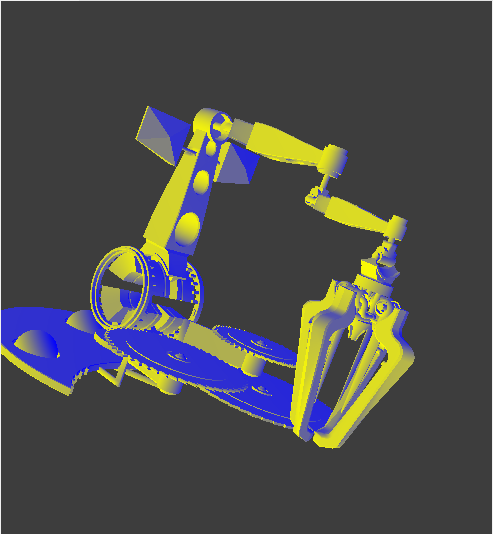
\includegraphics[scale = .6]{HW3_1_1.png}
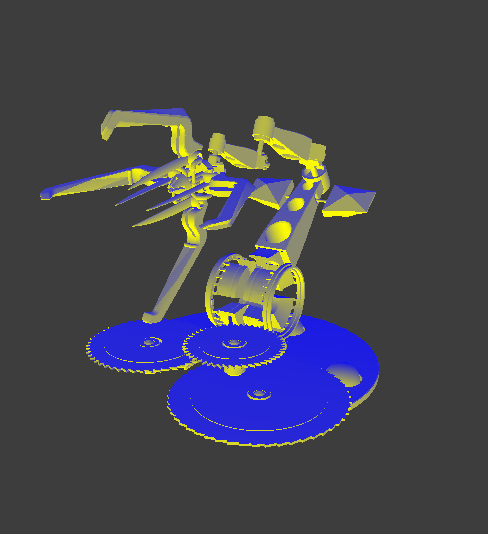
\includegraphics[scale = .6]{HW3_1_2.png}

\begin{verbatim}
void C5E3f_basicLight(float4 position  : TEXCOORD0,                        
                      float3 normal    : TEXCOORD1,

                  out float4 color     : COLOR,

              uniform float3 globalAmbient,
              uniform float3 lightColor,
              uniform float3 lightPosition,
              uniform float3 eyePosition,
              uniform float3 Ke,
              uniform float3 Ka,
              uniform float3 Kd,
              uniform float3 Ks,
              uniform float  shininess)
{
  float3 P = position.xyz;
  float3 N = normal;
  float3 L = P - lightPosition;
  float3 Blue = float3(0, 0, 1);
  float3 Yellow = float3(1, 1, 0);

  float ratio = (1 - dot(normalize(L), N))/2;
  float3 col = lerp(Blue, Yellow, ratio);

  color.xyz = col;
  color.w = 1;
}

\end{verbatim}

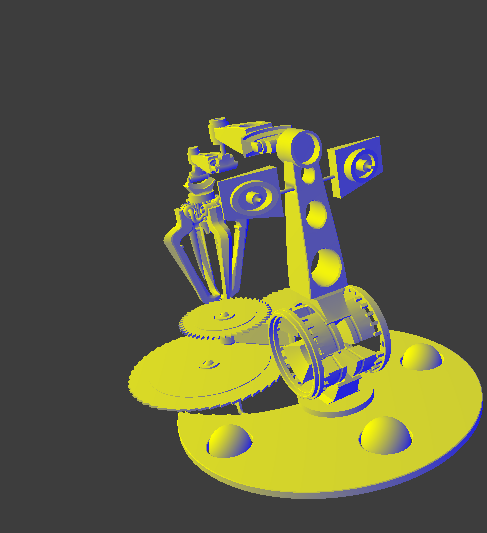
\includegraphics[scale = .6]{HW3_2_1.png}
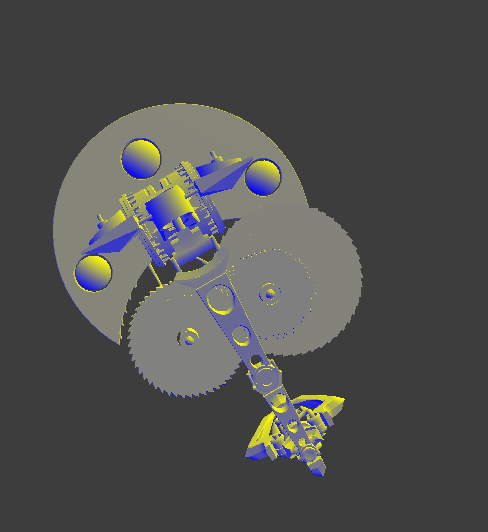
\includegraphics[scale = .6]{HW3_2_2.png}


\begin{verbatim}
void C9E2v_fog(float4 position    : POSITION,
                float4 color       : COLOR,
                float2 decalCoords : TEXCOORD0,

            out float4 oPosition    : POSITION,
            out float4 oColor       : COLOR,
            out float2 oDecalCoords : TEXCOORD0,
            out float  fogExponent  : TEXCOORD1,

        uniform float    fogDensity,  // Based on log2
        uniform float4x4 modelViewProj,
        uniform float4x4 modelView)
{	
  // Assume non-projective modelview matrix
  float3 eyePosition = mul(modelView, position).xyz;
  float fogDistance  = eyePosition.z;
  float s = -20;
  float e = -30;
  fogExponent  = max(0,min(1,(e - fogDistance)/(e-s)));
  oPosition    = mul(modelViewProj, position);
  oDecalCoords = decalCoords;
  oColor       = color;
}
\end{verbatim}

\begin{verbatim}
void C9E1f_fog(float2 texCoord    : TEXCOORD0,
               float  fogExponent : TEXCOORD1,
               float4 color       : COLOR,

           out float4 oColor : COLOR,

       uniform sampler2D decal,
       uniform float3 fogColor)
{
  float fogFactor   = fogExponent;
  float4 decalColor = tex2D(decal, texCoord);
  float4 texColor   = color*decalColor;

  oColor.xyz = texColor.xyz * fogFactor;
  oColor.w   = color.w;
}
\end{verbatim}

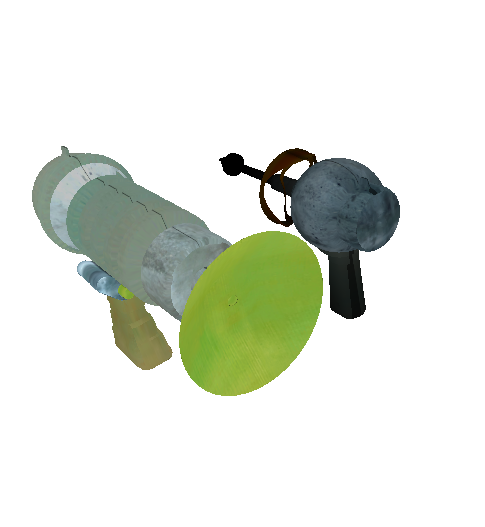
\includegraphics[scale = .6]{HW3_3.png}

\begin{verbatim}
float3 expand(float3 v) { return (v-0.5)*2; }

void C8E2f_bumpSurf(float2 normalMapTexCoord : TEXCOORD0,
                    float3 lightDir          : TEXCOORD1,
		    float3 lightPos	     : TEXCOORD2,

                out float4 color : COLOR,

            uniform sampler2D   normalMap)
{
  // Normalizes light vector with normalization cube map
  //texCUBE(normalizeCube, lightDir).xyz;
  float3 lightTex = normalize(lightDir).xyz;
  float3 light = expand(lightTex);
  // Sample and expand the normal map texture	
  float3 normalTex = tex2D(normalMap, normalMapTexCoord).xyz;
  float3 normal = expand(normalTex);

  //float3 origin = float3(0, 0, 0);
  float f = 2.0;
  // Diffuse lighting
  color = dot(normal,light);
  color *= pow((max(dot(normal, normalize(lightPos)), 0)), f);
}
\end{verbatim}

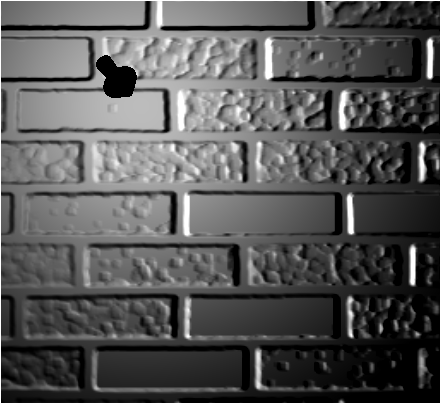
\includegraphics[scale = .6]{HW3_4.png}

\begin{verbatim}
struct C3E2v_Output {
  float4 position : POSITION;
  float4 color    : COLOR;
  float2 texCoord : TEXCOORD0;
};

float a = .03;
float b = 50;
float c = 10;

float d = .03;
float e = 50;
float f = 10;

C3E2v_Output C3E2v_varying(float2 position : POSITION,
                           float4 color    : COLOR,
                           float2 texCoord : TEXCOORD0,
			   uniform float time)
{
  C3E2v_Output OUT;

  OUT.position = float4(position, 0, 1);
  OUT.color    = color;
  OUT.texCoord.x = a * sin(b * texCoord.y) * sin(c * time);
  OUT.texCoord.y = d * sin(e * texCoord.x) * sin(f * time);
  //OUT.texCoord = texCoord;

  return OUT;	
}
\end{verbatim}

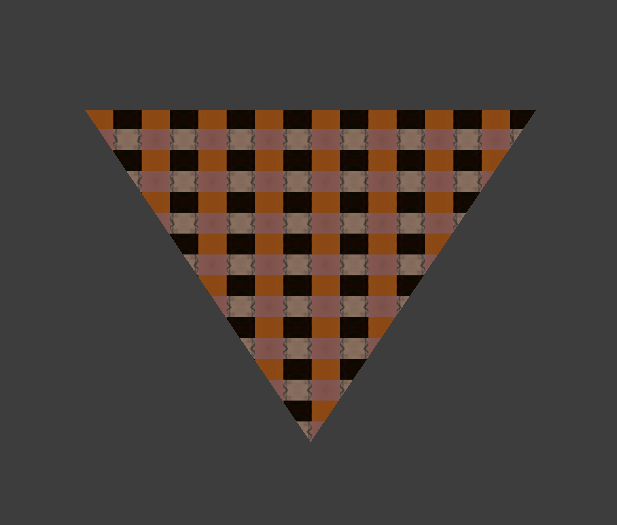
\includegraphics[scale = .6]{HW3_5.png}

\end{document}
